Data4Help Core is the central component of the system that connects all the other parts of the structure.
\begin{center}
    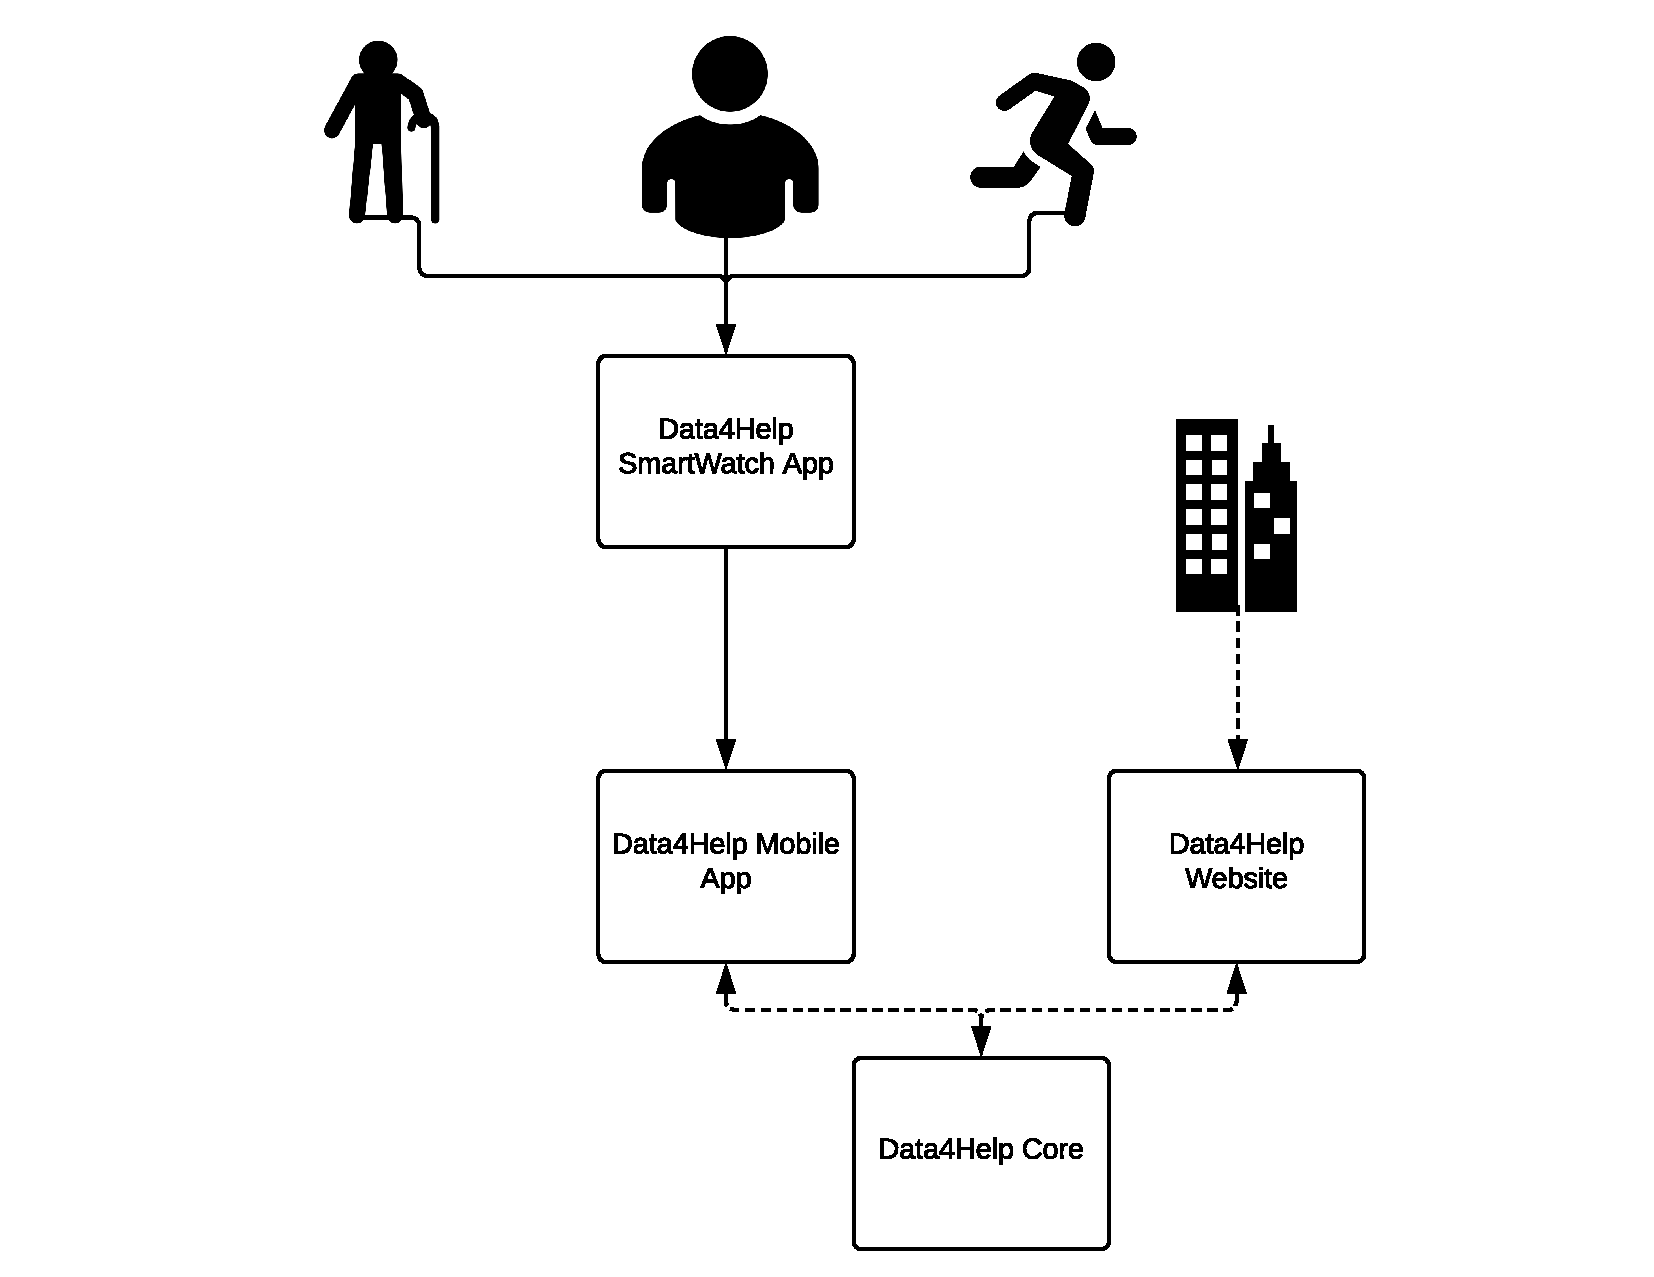
\includegraphics[height=7cm]{assets/useflow.pdf}
\end{center}

The Smartwatch App should be directly connected to the Mobile App to acquire data and let them be shown in the smartphone. In turn, the Mobile App has to communicate with the Data4Help Core that will register the data of the user. The Data4Help Website should communicate with the Data4Help Core as well in order to query directly on the company database.
\newline
\textbf{
TODO: 
A. Product perspective: here we include further details on the shared phenomena and a
domain model (\textbf{class diagrams and statecharts)}
}